\chapter{Core Features and Workflows}
\label{ch:features}

\begin{center}
\textit{This chapter explains each implemented feature area --- its purpose,
data model, workflow, and integration with the authorization model of
Chapter~\ref{ch:security}.}
\end{center}

\vspace*{\fill}
\clearpage
\section{Identity and Tenancy}

Users, institutes, memberships, roles, and permissions form the identity core.
There is no public self-registration: institute admins create users and
memberships, so every account arrives with an institute context and role. A
user may belong to several institutes; the client pins the active institute
(\texttt{x-institute-id}) per request and the browser stores it locally,
clearing it on logout or an unauthorized response. The membership picker
returns the user's memberships together with their resolved institute-domain
permission keys, so the web client can adapt its UI to what the user may
actually do. Institute lifecycle (create/deactivate) is modelled as
platform-plane work for a future \texttt{SUPER\_ADMIN} surface; role
management and user provisioning are institute-admin features today.

\section{Academic Structure and Academic Scope}

The academic module models \texttt{academic\_years}, \texttt{classes},
\texttt{divisions}, \texttt{subjects}, \texttt{chapters}, \texttt{topics}, and
the offering table \texttt{class\_subjects}. Teacher assignments bind a
membership to an offering (class--subject) for a term; student placements bind
a membership to a year--class--division and can be refined by explicit subject
enrollments. This structure is the input to
\texttt{\seqsplit{AcademicScopeService}}
(Figure~\ref{fig:academic-scope-resolution}): teachers and students get a
subject set
from their assignments/placements, from which every content query is scoped.
Structural administration (structure creation, assignment changes) is admin
work; content visibility derived from it is enforced per query.

\section{Materials and the OCR Pipeline}

\sectionmark{Materials and OCR}
Materials are uploaded as PDF, image, or document files (chunked upload for
large files, up to 20~MB total), or entered as plain text. Each material row
tracks \texttt{processing\_status} (\texttt{UPLOADED} $\rightarrow$
\texttt{QUEUED} $\rightarrow$ \texttt{PROCESSING} $\rightarrow$ \texttt{READY} |
\texttt{FAILED}) and a revision number.
Processing is asynchronous and coordinator-owned: the in-API coordinator
adopts queued \texttt{MATERIAL\_PROCESS} jobs, splits the source into page
chunks of default size ten, and lets registered OCR workers claim chunks under
a lease. Figure~\ref{fig:ocr-processing} and Figure~\ref{fig:ocr-processing-part2}
show the distributed flow and Figure~\ref{fig:ocr-state} and Figure~\ref{fig:ocr-state-part2}
the job/chunk state machines.

\begin{sidewaysfigure}[p]
\centering
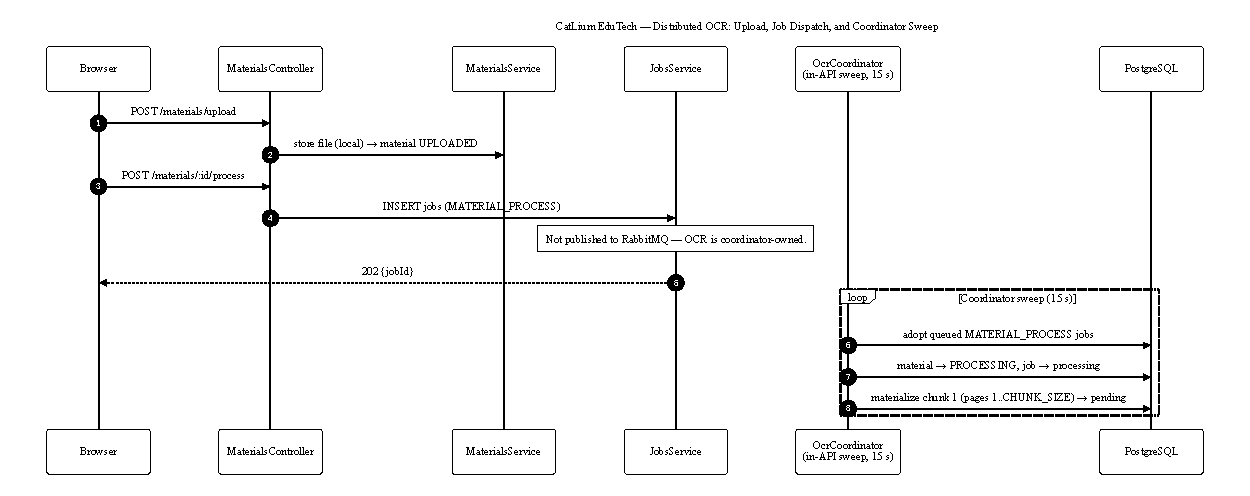
\includegraphics[width=711.5pt]{figures/ocr-flow-coordinator-sequence-bw.pdf}
\caption{Distributed OCR material processing, part 1: upload, job dispatch,
and the coordinator sweep.}
\label{fig:ocr-processing}
\end{sidewaysfigure}

\begin{figure}[p]
\centering
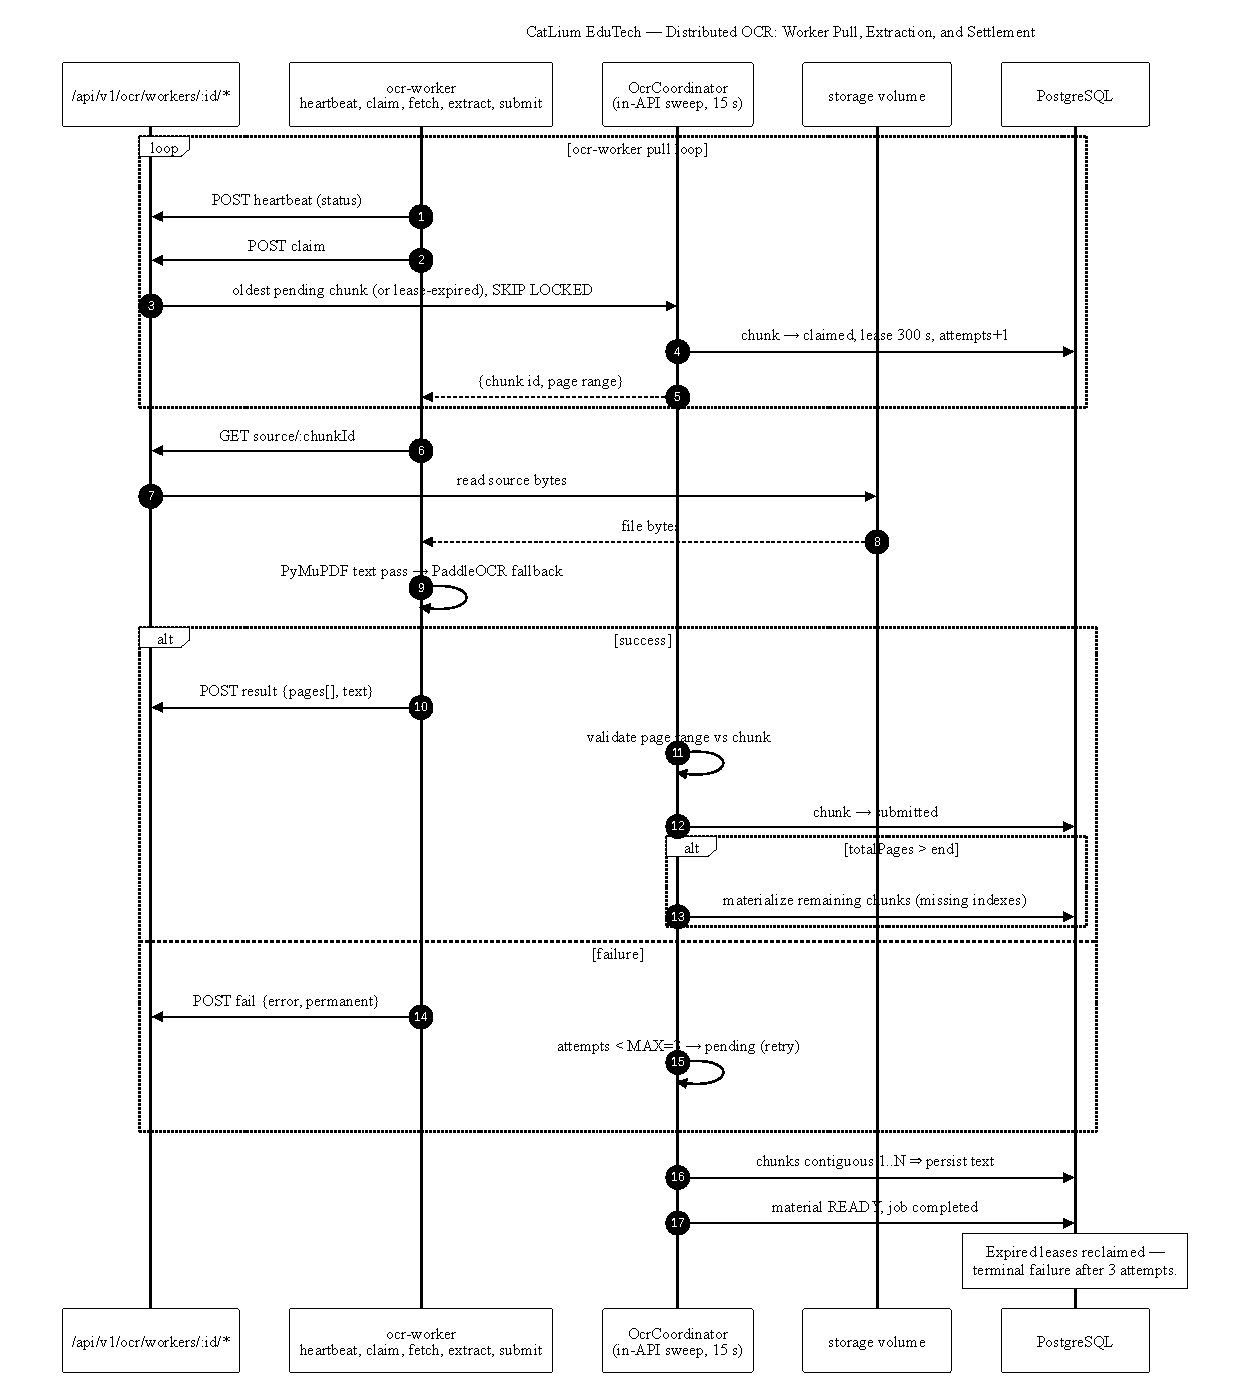
\includegraphics[width=436.5pt]{figures/ocr-flow-worker-sequence-bw.pdf}
\caption{Distributed OCR material processing, part 2: worker pull, extraction,
and settlement.}
\label{fig:ocr-processing-part2}
\end{figure}

\begin{sidewaysfigure}[p]
\centering
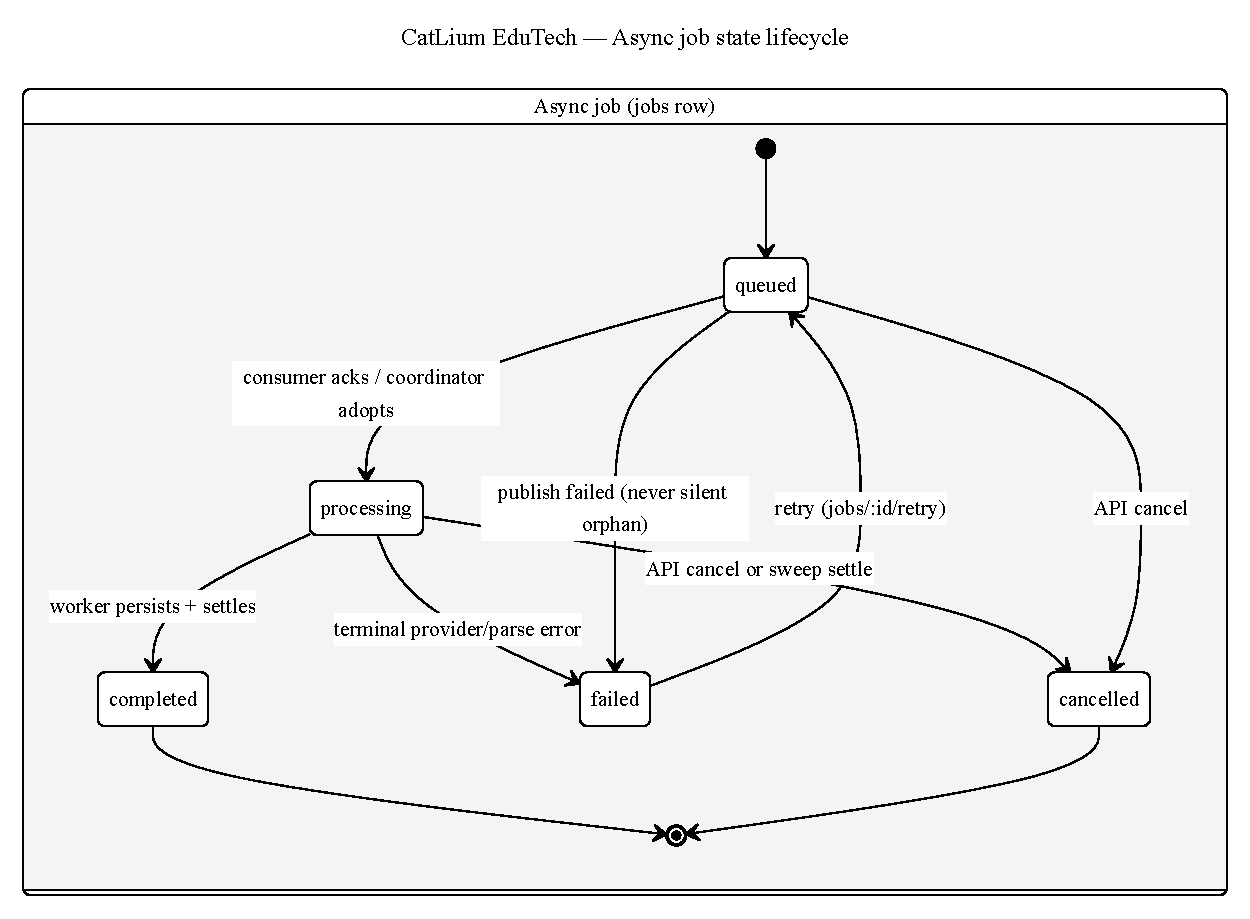
\includegraphics[width=544.9pt]{figures/state-job-lifecycle-bw.pdf}
\caption{Job state lifecycle.}
\label{fig:ocr-state}
\end{sidewaysfigure}

\begin{sidewaysfigure}[p]
\centering
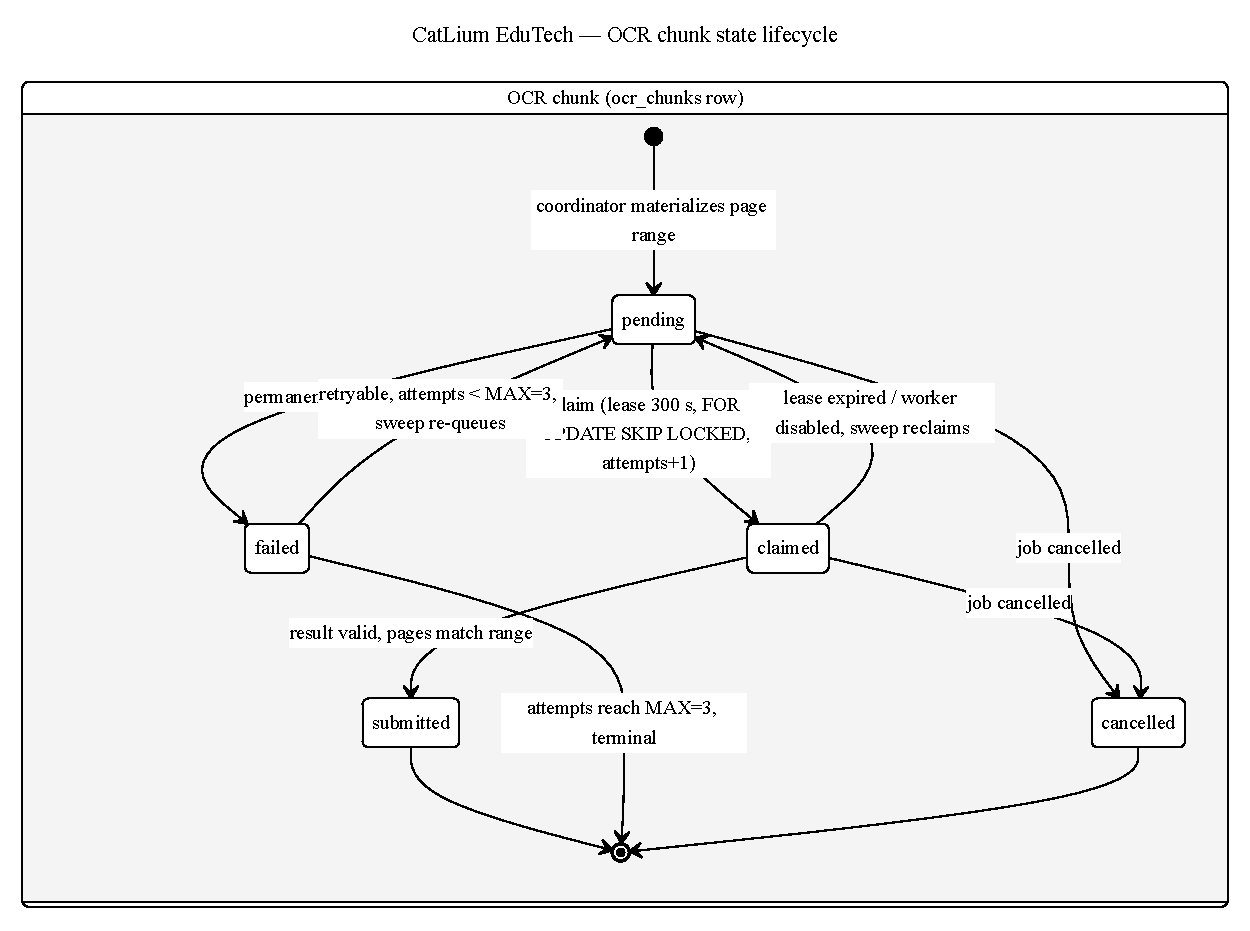
\includegraphics[width=537.6pt]{figures/state-chunk-lifecycle-bw.pdf}
\caption{OCR chunk state lifecycle.}
\label{fig:ocr-state-part2}
\end{sidewaysfigure}

For each page an OCR worker first tries PyMuPDF embedded text; a page with at
least five usable characters is accepted as-is, otherwise the page is
rasterised and fed to PaddleOCR. Extraction is followed by a deterministic
character-normalization pass. Worker claims are granted with
\texttt{FOR UPDATE SKIP LOCKED}; a lease (default 300 seconds) is renewed by
heartbeat, and the coordinator sweep (default every 15 seconds) reclaims
expired or disabled-worker claims, retries failed chunks while the attempt
count is below three, and settles cancellations. When all chunks of a
material are submitted and the pages are contiguous, the aggregate text is
persisted and the material becomes \texttt{READY}, which unlocks downstream
reuse: page-level text is viewable and users can submit per-page corrections
that re-apply over the extracted text. Workers authenticate per worker
(\texttt{owr\_...} keys against a SHA-256 hash); the worker-facing endpoints
are throttled and platform-gated.

\section{Syllabus Intelligence}

A syllabus document is uploaded (text or file) and processed to text, then
analysed by an AI job (\texttt{AI\_ANALYZE\_SYLLABUS}) that produces a
per-subject \texttt{structure} (chapters with their topics) and a
\texttt{context} (program, course, academic year, objectives, learning
outcomes, units and their scope). The lifecycle runs
\texttt{PROPOSED $\rightarrow$ CONFIRMED} (with \texttt{ARCHIVED}), and the
analysis can be re-run; a \texttt{CONFIRMED} syllabus is never silently
overwritten, so teachers can confirm a version and regenerate without data
loss. Each subject's syllabus carries a version number (\texttt{max+1} on
replacement) and both processing and analysis three-state machines.

\section{Material Intelligence (Deterministic Enrichment)}

In addition to AI, materials receive a deterministic structural enrichment
(\texttt{\seqsplit{material\_enhancements}}): a pure algorithmic pass over the extracted
pages that classifies every block (heading, paragraph, list, table, equation,
other) and keeps or marks segments (chapter/section) with a relevance level and
a confidence-scored mapping to syllabus topics. This pass is idempotent --- a
source fingerprint (checksum of extracted text and revision) prevents
duplicate re-enrichment --- and never modifies the raw extraction; excluded
blocks retain their original text and a reason. Enrichment is coordinator-owned
like OCR and triggered by OCR completion, corrections, text sources, or manual
re-enhancement.

\section{Study Content and AI Generation}

Content items are typed (\texttt{NOTE}, \texttt{\seqsplit{FLASHCARD\_SET}},
\texttt{\seqsplit{CORNELL\_NOTE}}, \texttt{SUMMARY},
\texttt{\seqsplit{IMPORTANT\_CONCEPTS}}), carry
a source (\texttt{MANUAL} | \texttt{AI\_GENERATED} |
\texttt{\seqsplit{OCR\_EXTRACTED}}
| \texttt{IMPORTED}), a status (\texttt{DRAFT} | \texttt{ACTIVE} |
\texttt{ARCHIVED}), and versioned payloads in \texttt{content\_versions} that
store the rendered HTML and AI context. Content availability is scoped by the
subject chain and the actor's academic scope.

AI generation (Figure~\ref{fig:ai-generation} and
Figure~\ref{fig:ai-generation-part2}) is an asynchronous pipeline:
the API writes a \texttt{jobs} row and publishes to the \texttt{ai\_generation}
queue; a Python worker with bounded concurrency resolves the eligible READY
source materials, assembles a bounded context budget, calls the model through
the OmniRoute gateway in chunks, validates each response against a strict
Pydantic schema for the requested artifact, aggregates and deterministically
de-duplicates, then persists the produced items AI-generated with provenance
(source type, source id, exact material revisions used). Generation on a topic
with no READY material enqueues a starter-material job whose
dependent-resources release the planned children, so a topic's generation
waits until it has usable sources. Generated content is versioned in place
(with REGENERATION change types) and never duplicated per topic/type.

\begin{sidewaysfigure}[p]
\centering
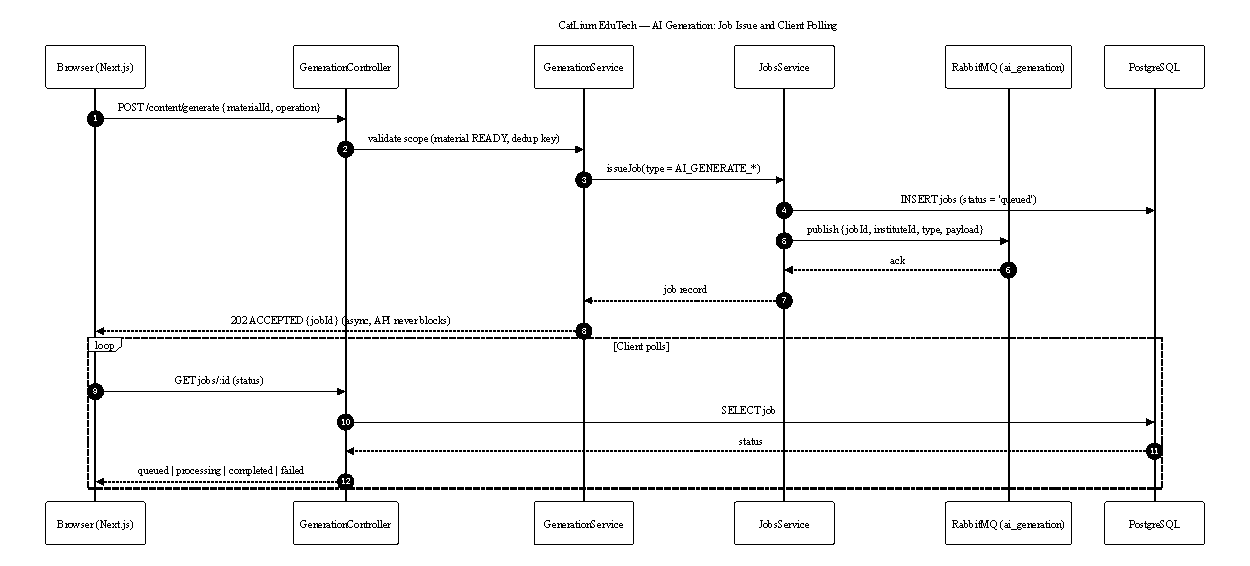
\includegraphics[width=711.5pt]{figures/ai-generation-issue-sequence-bw.pdf}
\caption{Asynchronous AI generation, part 1: job issue and client polling.}
\label{fig:ai-generation}
\end{sidewaysfigure}

\begin{sidewaysfigure}[p]
\centering
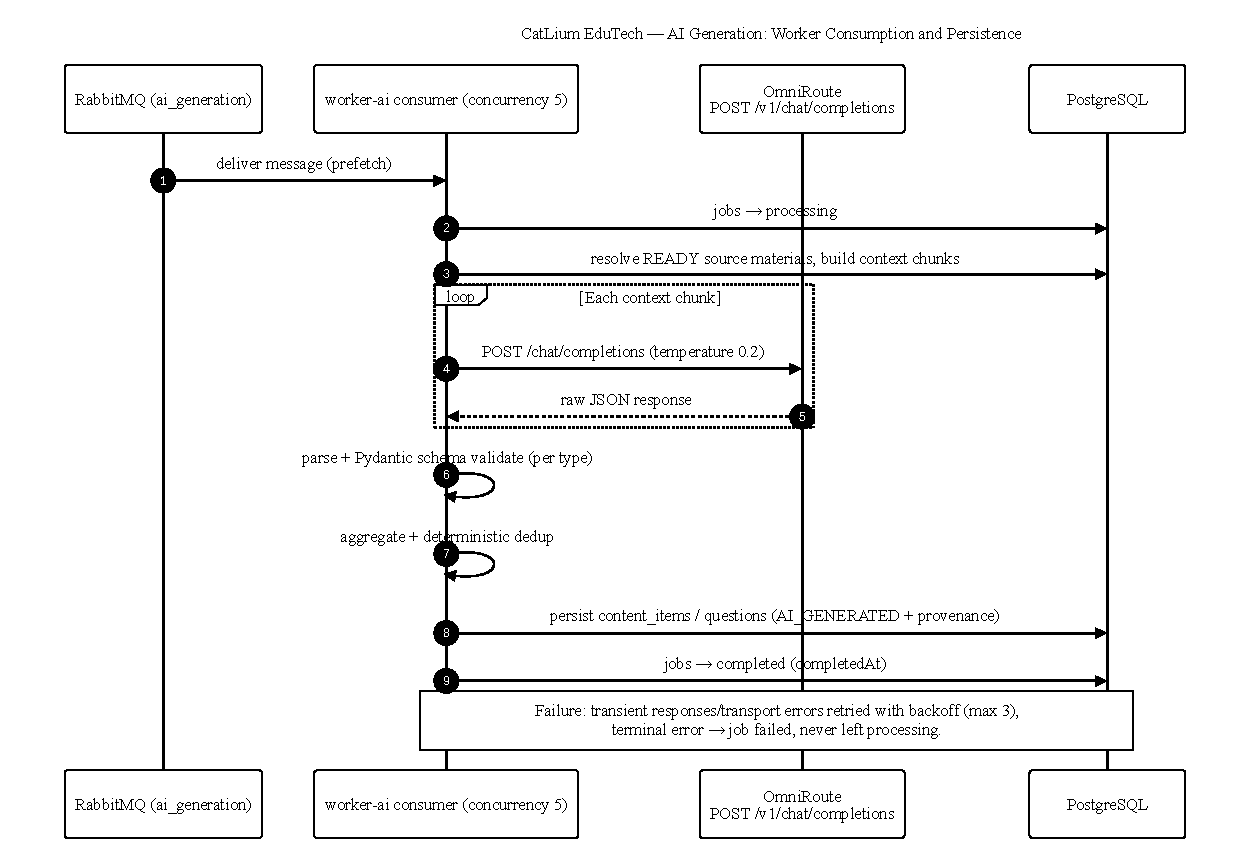
\includegraphics[width=580.4pt]{figures/ai-generation-consume-sequence-bw.pdf}
\caption{Asynchronous AI generation, part 2: worker consumption, OmniRoute
calls, and persistence.}
\label{fig:ai-generation-part2}
\end{sidewaysfigure}

\section{Question Types and the Question Bank}

\sectionmark{Question Bank}
Question types are \emph{data}: the seeded global starters cover
\texttt{MCQ}, TRUE/FALSE, FILL-IN-BLANK, DEFINITION, VERY-SHORT/SHORT/BRIEF/LONG
answer, MATCH-THE-FOLLOWING, CASE-STUDY, and NUMERICAL types, and institutes
may define custom types with their own instructions and defaults. Each type
carries an \texttt{answer\_format} (\texttt{MCQ} | TRUE\_FALSE | FILL\_IN\_BLANK |
TEXT | MATCHING | NUMERICAL) and an objective/subjective kind; the format is
copied onto each question at write time so validation and evaluation always
know the shape of the answer.

The question bank \emph{is} the \texttt{questions} table: stems are scoped to a
subject (optionally chapter/topic), carry difficulty, explanation, an
approval state (\texttt{PENDING} only for staging; new questions are
\texttt{APPROVED}), a source, and provenance. Generation can target a single
type or a full \emph{bank bucket} plan built from question types and a
difficulty distribution (default 34/33/33 across EASY/MEDIUM/HARD), with
per-type minima raised to the type's floor and exact-sum allocation by the
largest-remainder method. Generation is pattern-aware: \texttt{ensurePatternCoverage}
reports COVERED, AWAITING\_APPROVAL, INSUFFICIENT, or GENERATING and queues
exactly the deficit when generating. The worker de-duplicates identical stems
within a batch and inserts questions directly as APPROVED+ACTIVE. Bank
analytics (total/usable, by type, by difficulty) and set management complete
the surface.

\section{Paper Patterns (Blueprints)}

A paper pattern is a blueprint: a title, a subject set
(\texttt{paper\_pattern\_subjects}), a status lifecycle
(\texttt{DRAFT $\rightarrow$ REVIEW $\rightarrow$ APPROVED}), an optional
locked flag, a version, a source type (\texttt{MANUAL}, \texttt{TEXT},
\texttt{MATERIAL}, \texttt{PREVIOUS\_YEAR\_PAPER}), and a structural JSONB that
declares up to 50 sections, each with rules for question type, counts, marks,
compulsoriness, attempt counts, and difficulty/topic distributions. Fields
left \texttt{null} are explicitly \emph{unknown}, never fabricated. Patterns
can be analysed by AI to draft a \texttt{REVIEW} blueprint from a source, and
validated deterministically (the validate endpoint returns
\texttt{\{valid, errors\}}); only \texttt{APPROVED} patterns drive generation
or assessment creation, and approval auto-locks the blueprint. Deterministic
extraction of a pattern from an uploaded source file creates the pattern
immediately and then runs a queued extraction job. Access is staged: DRAFT and
REVIEW are owner-and-admin, APPROVED is pure academic scope.

\section{Question Papers}

A question paper is a fixed snapshot selection of bank questions against a
pattern for student-facing distribution. It stores a scope, instructions,
duration, max marks, and a junction (\texttt{question\_paper\_questions}) that
freezes marks, sections, and sort order at selection time so exports stay
stable. Selection from a pattern replaces the set and re-applies the pattern
rules; coverage computation reports OK, SHORT, EXCESS, or TYPE\_MISMATCH, and
an underserved paper can generate exactly the missing items. A paper converts
to a DRAFT assessment by copying its junction, without re-selection. Papers
may also be produced by deterministic extraction from a source document, with
candidate questions placed in a shared review tray.

\section{Assessments and Attempts}

Assessments are authored resources with a title, scope, timing
(\texttt{starts\_at}/\texttt{ends\_at}), duration, max marks, instructions, and
an explicit state machine \texttt{DRAFT $\rightarrow$ PUBLISHED $\rightarrow$
ACTIVE $\rightarrow$ COMPLETED}, with an unpublish transition DRAFT-ward while
not started. Authoring restricts edits to DRAFT; the publish action re-checks
every link is APPROVED and ACTIVE, that the assessment is scoped and timed, and
that its blueprint coverage is sufficient. Questions can be linked directly or
auto-selected from an approved pattern by type and difficulty. A completed
assessment is terminal.

\subsection{Attempts and evaluation}

An attempt is a timed, snapshot-based student response:
\begin{itemize}
  \item \textbf{Start} is allowed for a published/active assessment within its
  schedule window, with one in-progress attempt per student (enforced by a
  partial unique index and surfaced as \texttt{409}). The full question set is
  snapshotted server-side (stem, type, format, marks, payload); the student
  view is sanitized so answer keys are never sent before answering.
  \item \textbf{Answer saving} validates the answer against its format (for
  example, an MCQ choice id must exist in the choices) and upserts on the
  unique attempt-question pair, guarded by \texttt{FOR UPDATE} on the attempt.
  \item \textbf{Deadline expiry} is enforced server-side: a past-deadline
  in-progress attempt is atomically transitioned to \texttt{EXPIRED} and
  evaluated in the same transaction, so it is never observable as both
  terminal and unevaluated.
  \item \textbf{Evaluation} dispatches on the answer format for the objective
  formats (MCQ, true/false, fill-in-the-blank, matching, numerical). Text and
  custom answers are recorded but never auto-graded (the marker records zero
  marks for them); this keeps the scoring contract honest and defers
  essay-grade automation to the checking-system scope.
  \item \textbf{Submission} is idempotent; the result endpoint reveals
  correctness and awarded marks only for the student's own terminal attempt,
  and the analysis surfaces are aggregate (score distribution, per-question
  accuracy, topic and difficulty performance) with no student-level answer
  data leakage.
\end{itemize}

\section{Practice}

Practice is deliberately ungraded. \texttt{practice\_sessions} run in
\texttt{FLASHCARD} or \texttt{QUESTION} mode: flashcards show card backs from
a content item; question mode presents bank questions. Each session snapshots
its items at start (sanitized), and a per-item response records an
\texttt{AGAIN}/\texttt{GOOD} rating (flashcard) or the answer plus a
correctness flag (question) computed by the same graded dispatcher --- but there
is no score, no ledger, and no analytics. Feedback is instant and per-item:
the answer key is revealed only after the item is answered, in-session. One
open session per source is enforced, and sessions complete idempotently.

\section{Exports}

All export routes share one visual model --- a document of typed blocks
(headings, paragraphs, bullets, steps, flashcards, questions, tables,
formulas, examples, callouts, timelines, diagrams, further-learning lists) ---
from which the PDF, DOCX, and XLSX renderers and the web preview draw. PDF is
produced with real Chromium via a shared lazy browser; DOCX with a document
library; XLSX with a small dependency-free worksheet writer (one worksheet per
table block). Question exports are arranged either by rank order for teacher
sets or by the pattern's section order for pattern-based papers; a
\texttt{paper}/\texttt{answers} flag toggles student-facing (no answers) versus
teacher (answer-key) renderings. Every export/preview route is explicitly
restricted to institute admins and teachers and evaluates academic scope
through the authoritative read gate of the source module, resolving out-of-scope
requests to \texttt{404}.

\section{Asynchronous Job Lifecycle}

All of the above heavy operations ride the generic job subsystem
(\texttt{jobs}): \texttt{queued $\rightarrow$ processing $\rightarrow$
completed | failed | cancelled}, plus a transient \texttt{cancelling} for
in-flight work. Jobs are tenant-scoped, carry their requester for
accountability, and may be retried when failed or cancelled. Coordinator-owned
job types (OCR/enhancement/extraction) are never published to the broker and
are adopted by the sweep; AI and extraction types are reserved to guarded
paths. Publication failures mark the job failed rather than leaving a silent
orphan, and a partial unique index prevents duplicate live generation jobs per
source.